% status: 75
% chapter: TBD

\def\paperstatus{75} % a number from 0-100 indicating your status. 100
                % means completed
\def\paperchapter{TBD} % This section is typically a single keyword. from
                   % a small list. Consult with theinstructors about
                   % yours. They typically fill it out once your first
                   % text has been reviewed.
\def\hid{hid-sp18-705} % all hids of the authors of this
                                % paper. The paper must only be in one
                                % authors directory and all other
                                % authors contribute to it in that
                                % directory. That authors hid must be
                                % listed first
\def\volume{9} % the volume of the proceedings in which this paper is to
           % be included

\def\locator{\hid, Volume: \volume, Chapter: \paperchapter, 
	Status: \paperstatus. \newline}

\title{New Approaches to Managing Metadata at Scale in Research Libraries}
\author{Timothy A. Thompson}
\affiliation{%
  \institution{Indiana University Bloomington}
  \streetaddress{School of Informatics, Computing, and Engineering}
  \city{Bloomington} 
  \state{Indiana} 
  \postcode{47408}
}
\email{timathom@indiana.edu}

\begin{abstract} 
The analysis of big data often relies on distributed storage and
computation; however, access to big data---and to the platforms capable of
managing and processing it---continues to be largely centralized.
Centralization is particularly evident in the case of the metadata produced,
managed, and disseminated by academic and research libraries. Libraries
typically create and share their catalog records by uploading them to a
centrally managed database, which can then be searched by other libraries for
records that can be copied and added to an institution's local catalog. This
centralized approach, which operates on the basis of membership fees, has the
advantage of scalability and availability, but it comes at the cost of a loss
of autonomy. Although technical innovation is possible within the current
paradigm, the growing maturity of peer-to-peer protocols and decentralized
solutions points toward an alternative approach, one that would allow
libraries to share their data directly without having to pay an expensive
intermediary.
\end{abstract}

\keywords{i523, hid-sp18-705, Research Libraries, Library Catalogs, 
Peer-to-Peer, Blockchain}

\maketitle

\section{Introduction}
The problem of entity resolution (also known as record linkage or data
matching~\cite{pC12}) is one that has a direct impact on the work of
information professionals in research libraries. In library units
responsible for catalog management, many workflows center on a procedure
known as copy cataloging, which aims to expedite the processing of new
acquisitions. Copy cataloging involves searching a shared database for
records created by another cataloging agency, but that describe identical
publications that have been acquired by one's local institution~\cite{cD17}.
In the current environment, a single company, the Online Computer Library
Center (OCLC---\url{http://www.oclc.org}), is the only viable platform for
global cooperative cataloging~\cite{aT10}. OCLC provides data aggregation
and warehousing services that allow libraries to effectively share their
data, but its business model does not encourage peer-to-peer interaction and
innovation among individual libraries. This vendor-driven paradigm entails
the acceptance of a business model that, in effect, charges libraries for
serving their own data back to them, with some added value through quality
control and normalization. Once a library's data has been sent to OCLC, it
also becomes subject to potential licensing restrictions, as well as the
expectation that future dissemination of the data will include attribution
of OCLC~\cite{oclcND, oclc10}.

\section{New Approaches to Metadata Management}
Libraries have a tradition of experience with record matching and
automation~\cite{jM92}, but now stand to benefit from the increasingly
mainstream availability of algorithms and routines developed within the
context of data science and machine learning. Sophisticated algorithms for
string comparison and probabilistic record linkage have long been
available, but are not widely used by libraries, with the exception of
large-scale projects such as the Social Networks and Archival Context
Project (SNAC) (\url{http://snaccooperative.org/}) and the Virtual
International Authority File (VIAF) (\url{http://viaf.org/}). The former has
employed methods based on Naive Bayes classification algorithms to aggregate
and disambiguate data from across a wide range of libraries and archives
(the reported accuracy of the approach fell with the range of 80-90
percent)~\cite{rL11}. More recent approaches to record matching have
improved on probabilistic methods such as Naive Bayes by using Artificial
Neural Networks, improving accuracy rates in some cases to 98 percent or
more~\cite{rG17}.

As machine learning tools and methods have become more accessible,
however, large-scale, real-time access to library metadata has not
necessarily followed suit. The catalog of a large academic library may
contain around 10 million records~\cite{yul18}. By comparison, as of August
2018, the OCLC catalog database, WorldCat, contained 427,501,671
bibliographic records in 491 languages~\cite{oclc18}. As long as service
providers such as OCLC maintain centralized control over the aggregated
metadata of research libraries, large-scale computational analysis---and the
innovation it could produce---will remain proprietary and locked away.

The situation is further complicated by professional and cultural norms
within libraries. Although decentralization may be appealing as an ideal,
librarians who manage bibliographic metadata are also immersed in a
discourse that centers on the idea of control: they use terms such as
authority control, controlled vocabularies, and intellectual and physical
control of collections~\cite{olson01}. The idea of control is closely
related to the idea of trust: when workflows and systems are centralized, it
becomes easier to enforce norms and standards, but it also becomes more
likely that potential contributors may be excluded, especially when they are
unable to afford the price of membership in a proprietary system.

New distributed technologies and protocols, including blockchains and
distributed hash tables (DHTs), could allow research libraries to form
robust peer-to-peer networks that would enable data sharing on a larger
scale. Although public blockchains such as Ethereum and Bitcoin are limited
in the amount of data that can feasibly be stored on chain, alternative
platforms that address this limitation have recently emerged. The
blockchain-based database service BigchainDB, implemented in Python,
provides a robust storage data solution while preserving the benefits of
blockchain features such as data immutability and an asset-based
transactional model. By running a consortium blockchain network of
BigchainDB nodes~\cite{vButerin15}, libraries could be empowered to abandon 
centralized models and begin managing their data collectively.

\section{Blockchains for Research Libraries}
Some in the library profession have been skeptical of blockchain
applications for their domain, arguing that they have been overhyped as a
panacea, when in reality they are nothing more than slow, expensive,
append-only databases~\cite{sjsu18}. Even core developers working to support
the Bitcoin blockchain have argued that the constraints imposed by
blockchain technology, such as immutability and decentralized consensus,
make it appropriate for a very limited set of applications---namely,
currency and the exchange of value~\cite{jSong18}. For individuals and
organizations who are investigating blockchains as a technical solution, it
is important from the outset to establish a framework for evaluating their
applicability and appropriateness~\cite{bS28}. For example, a
blockchain-based solution may be appropriate in a scenario in which there is
a lack of trust among participants, or in which processes and collaboration
would be more efficient if the need for trust were eliminated~\cite{bS28}.
In the case of a shared catalog for research libraries, trust is an issue
because not all participants can be trusted to provide data that conforms to
expected levels of quality. A commercial, centralized solution mitigates
these concerns by requiring participants to pay a membership fee. A
blockchain solution addresses issues of trust by enforcing a decentralized
consensus mechanism, which may take different forms, but which is designed
to ensure that participants can trust the network to maintain a consistent
state across all transactions~\cite{buchman2018latest}.

The Proof-of-Stake consensus algorithm, employed by some blockchain
networks as an alternative to Bitcoin's resource-intensive Proof-of-Work
mechanism, is similar to the membership fee model in that validator nodes
are elected based on their share of ``stake'' in the network, measured by
their willingness to commit or stake an allocation of network tokens as a
proof of honesty~\cite{gMarin18}. For research library applications, a
variation of Proof-of-Stake known as Proof-of-Authority may be the most
appropiate solution~\cite{gMarin18, vButerin15}. In contrast to public
blockchains such as Ethereum and Bitcoin, or fully private blockchains
restricted to a single organization, so-called consortium blockchains may be
the preferred approach, one in which consensus ``is controlled by a
pre-selected set of nodes''~\cite{vButerin15}. The model implemented by the
BigchainDB project fits the parameters of a consortium blockchain that
implements a Proof-of-Authority approach to consensus~\cite{bdb18b}.

\section{Design Requirements}
A blockchain-based catalog for research libraries should support the
creation of a decentralized marketplace for library metadata. Rather than
paying a centralized exchange to distribute their catalog records, libraries
could buy and sell records in a peer-to-peer exchange. Catalog records could
thus become a source of revenue rather than a costly expenditure. Many
blockchain systems support the creation of so-called smart assets, or the
creation of tokens to represent real-word assets. A new token could be
minted to facilitate the exchange of metadata objects, and payment and
settlement channels could be created using smart contracts on a public
blockchain such as Ethereum. However, a public blockchain solution does not
fully satisfy the requirements of decentralization for this use case. A data
asset cannot be represented exclusively by a token---it also needs to be
stored in a decentralized system optimized for read and write transactions.
Public blockchains such as Ethereum have been designed for exchange, not
storage. At the current price of the Ethereum blockchain's native token,
Ether (ETH), at approximately \$200.00, storing 1 Gigabyte of data on the
blockchain would cost over \$7,000,000.00~\cite{tHess16}. A decentralized
system for library metadata must be able to scale and store big data out of
the box. BigchainDB is a production-ready solution that meets the
requirements for this use case: it supports the creation of tokens and the
direct storage of metadata objects on its
blockchain~\cite{bdb18c}.

\section{Project Scope}
The current project presents findings from an exploration of BigchainDB as a 
blockchain database solution for a shared library catalog. It includes a 
preliminary analysis of library metadata requirements and whether they can be 
satisified using BigchainDB.

\section{BigchainDB}
\subsection{Evolution}
BigchainDB arose as an attempt to address the scalability and storage
limitations of traditional blockchains such as Bitcoin and Ethereum and to
create a hybrid solution that builds a blockchain layer on top of an
existing big data system~\cite{bigDB18}. Development of the BigchainDB
framework initially focused on integration with the RethinkDB system
(\url{https://www.rethinkdb.com/}), but now works exclusively with MongoDB
(\url{https://www.mongodb.com/})~\cite{ks16, bigDB18}.

The early focus of BigchainDB development was to create an
architecture that would allow existing big data databases to be
``blockchainified''~\cite{bigDB16a}. The original BigchainDB whitepaper,
released in June 2016, focused on the scalability limitations of traditional
blockchain networks such as Bitcoin and claimed that it should be possible
to develop a blockchain-based distributed database that would enable ``1
million writes per second throughput, storing petabytes of data, and
sub-second latency''---in contrast to the storage restrictions and 7
transaction-per-second (tps) limit of the Bitcoin network~\cite{bigDB16a}.
The advantages of adding a blockchain layer to an existing distributed
database would be to incorporate ``decentralized control, immutability, and
creation [and] movement of digital assets''~\cite{bigDB16a}. 

The primary challenge in designing a decentralized system is how to
defend against both arbitrary failure and malicious actors. In so-called
Sybil attacks, an attacker attempts to generate false identities in order to
gain majority control over a network~\cite{dJ02}. To address Sybil attacks,
BigchainDB proposes a governance model that would create a federation of
trusted nodes. Because all participants are known, any attempt by one
participant to gain control over the network would be obvious. A more
pervasive vulnerability comes in the form of the so-called Byzantine
Generals' Problem~\cite{bigDB16a}. Nodes in a distributed network must be
able to reach consensus about the final order of transactions at each state
of the system, even in the presence of node failure or malicious attempts to
manipulate system state in order to gain an unfair advantage---for example,
in double-spending, in which a transaction is replayed so that the same
asset can be used again (a particular problem in the case of financial
transactions)~\cite{bigDB16a, aA17}.

In its original design, BigchainDB relied on the consensus algorithm of
its underlying database to manage benign node failure and incorporated
additional constraints to verify the integrity of the voting process by
which nodes in the network approved transactions---and the blocks containing
them---as valid~\cite{bigDB16a}. However, in its initial version, BigchainDB
did not claim to be Byzantine Fault Tolerant (or BFT---the term used to
indicate that a system can withstand unexpected node behavior, whether
benign or malicious, up to a certain threshold~\cite{bigDB16a}). In the
original design, all nodes belonged to a single logical database. This made
the system overly centralized and vulnerable to attack: a malicious actor
who gained control over a single node would be able to drop the entire
database, which was shared among all nodes in the network~\cite{ks16, bigDB18}.
BigchainDB 2.0, released in June 2018, underwent a complete redesign and
incorporated full Byzantine fault tolerance through integration with
Tendermint, an application for managing consensus and state machine
replication in blockchain systems~\cite{troyM18b, tender18}. As a result of
implementing Byzantine fault tolerance through Tendermint, BigchainDB's
original goal of supporting 1 million tps was no longer viable. A recent
benchmark of BigchainDB 2.0 throughput performed by the BigchainDB team
indicated that the system was able to process approximately 300
tps~\cite{troyM18a}.

\subsection{Architecture}
The architecture of a BigchainDB 2.0 network is shown in
Figure~\ref{f:bdb}. Each node in the network is self-contained and
includes its own MongoDB database and Tendermint application server.
Tendermint is used to manage consensus, communication, and state replication
among nodes, whereas the software that is unique to BigchainDB is
responsible for ``registering and tracking the
ownership of `assets'\thinspace''~\cite{troyM18b}. In BigchainDB 2.0, as is
the case in general with systems that are Byzantine Fault Tolerant, $3f + 1$
nodes are necessary to run a network, where $f$ is the number of faulty
nodes to be tolerated~\cite{bdb18}. Therefore, at least four nodes are
required in order to run a BigchainDB network: if one of the four nodes
becomes unresponsive or attempts to approve an invalid transaction, the
network will continue to function based on the majority consensus of the
other three nodes~\cite{bdb18}.

A BigchainDB client can potentially connect to any node in the network.
Each MongoDB instance contains a full replication of the data stored in the
network~\cite{bdb18}. The BigchainDB project officially supports three
client drivers to connect to a node server (in Python, Node.js, and
Java)~\cite{bdb18f}.

\subsubsection{BigchainDB Server}
The BigchainDB Server, written in Python, implements the logic to
model, construct, validate, and store transactions in the BigchainDB
blockchain~\cite{troyM18b}. The server also incorporates a Python
implementation of the Crypto-Conditions specification, which is a standard
for enforcing complex boolean conditions for fulfillment (asset transfer)
using cryptographic signatures~\cite{cryptocon}.

All objects in BigchainDB are modeled as \emph{assets}. Two transaction types 
are available for managing assets: CREATE and TRANSFER~\cite{troyM18c}. Each 
transaction must be cryptographically signed with the private key of its 
``owner'' (the agent who created an asset through a CREATE transaction or to 
whom an asset was assigned through a TRANSFER transaction). Public/private 
keypairs are implemented using the Edwards-curve Digital Signature Algorithm 
Ed25519~\cite{troyM18c}. A transaction is encoded using a dictionary or 
associative array that can be serialized as a JSON object. The BigchainDB 
Transactions Specification defines the structure and usage of a BigchainDB 
transaction object~\cite{troyM18c}. Valid transactions must include the 
following keys:

\begin{verbatim}
{
    "id": ctnull,
    "version": version,
    "inputs": inputs,
    "outputs": outputs,
    "operation": operation,
    "asset": asset,
    "metadata": metadata
}	
\end{verbatim}

Conditions for fulfillment and asset transfer are defined in the values
of the ``inputs'' and ``outputs'' keys. An object representing the asset
itself is stored as the value of the ``asset'' key and cannot be modified
once an asset has been created and committed to a block in the BigchainDB
blockchain. The ``metadata'' key is used to store an arbitrary object that
records additional information about the asset or its state: in contrast to
the asset object, the metadata object \emph{can} be modified with each
TRANSFER transaction~\cite{troyM18c}.

\subsubsection{Tendermint}
Tendermint is a BFT consensus engine for blockchain applications. It
implements a set of protocols and exposes an interface (called the
Application Blockchain Interface---ABCI) for replicating deterministic
finite state machines~\cite{tender18}. 

\subsubsection{MongoDB}
MongoDB is an enterprise-grade NoSQL database optimized for storing
JSON objects as documents. It supports both high availability (replication)
and scalability (sharding)~\cite{mongo18}. Early verions of BigchainDB used
a single MongoDB replication set and were able to take advantage of these
core MongoDB features. In BigchainDB 2.0, because each node maintains a
separate MongoDB instance, replication and sharding are not supported out of
the box~\cite{troyM18b}. In order to enforce practical immutability and
decrease the likelihood of data tampering, the BigchainDB server limits
access to MongoDB and does not expose any interfaces for deleting or making
arbitary modifications to database documents. Although it is technically
possible for a systems administrator to modify the MongoDB database
directly, each BigchainDB transaction is signed with a public/private
cryptographic keypair---thus any tampering would result in a modified
signature, which would be detectable by other nodes in the network and would
violate its social contract~\cite{bigDB18}.

BigchainDB does take advantage of MongoDB's query facility for
read-only queries. It exposes a simple search interface through its HTTP
API, but also allows node administrators to create custom indexes and
leverage the full range of MongoDB query
functionality~\cite{bdb18d}.


\section{Dataset}
Lorem ipsum dolor sit amet, consectetur adipiscing elit. Sed sodales
eleifend pharetra. Phasellus interdum augue nec sapien pretium accumsan.
Proin dapibus massa in enim pulvinar facilisis. Proin venenatis nisl metus,
nec tincidunt lorem viverra at. Quisque sagittis lectus a mi varius, a
auctor tortor dapibus. Nam magna ex, rutrum et mauris et, eleifend iaculis
enim. Sed non tortor quis ligula placerat lacinia. Proin consectetur, sapien
quis molestie volutpat, velit lacus faucibus quam, id rutrum dui est et
eros. Ut fermentum malesuada hendrerit. Lorem ipsum dolor sit amet,
consectetur adipiscing elit. Fusce tempus, ante at suscipit facilisis,
mauris urna auctor urna, eget pretium mi massa accumsan massa. Duis semper,
ex eu rhoncus elementum, est est tristique est, nec tristique orci nunc eget
nibh. In vestibulum purus at nibh egestas, eget convallis mi molestie.

Lorem ipsum dolor sit amet, consectetur adipiscing elit. Sed sodales
eleifend pharetra. Phasellus interdum augue nec sapien pretium accumsan.
Proin dapibus massa in enim pulvinar facilisis. Proin venenatis nisl metus,
nec tincidunt lorem viverra at. Quisque sagittis lectus a mi varius, a
auctor tortor dapibus. Nam magna ex, rutrum et mauris et, eleifend iaculis
enim. Sed non tortor quis ligula placerat lacinia. Proin consectetur, sapien
quis molestie volutpat, velit lacus faucibus quam, id rutrum dui est et
eros. Ut fermentum malesuada hendrerit. Lorem ipsum dolor sit amet,
consectetur adipiscing elit. Fusce tempus, ante at suscipit facilisis,
mauris urna auctor urna, eget pretium mi massa accumsan massa. Duis semper,
ex eu rhoncus elementum, est est tristique est, nec tristique orci nunc eget
nibh. In vestibulum purus at nibh egestas, eget convallis mi molestie.

Lorem ipsum dolor sit amet, consectetur adipiscing elit. Sed sodales
eleifend pharetra. Phasellus interdum augue nec sapien pretium accumsan.
Proin dapibus massa in enim pulvinar facilisis. Proin venenatis nisl metus,
nec tincidunt lorem viverra at. Quisque sagittis lectus a mi varius, a
auctor tortor dapibus. Nam magna ex, rutrum et mauris et, eleifend iaculis
enim. Sed non tortor quis ligula placerat lacinia. Proin consectetur, sapien
quis molestie volutpat, velit lacus faucibus quam, id rutrum dui est et
eros. Ut fermentum malesuada hendrerit. Lorem ipsum dolor sit amet,
consectetur adipiscing elit. Fusce tempus, ante at suscipit facilisis,
mauris urna auctor urna, eget pretium mi massa accumsan massa. Duis semper,
ex eu rhoncus elementum, est est tristique est, nec tristique orci nunc eget
nibh. In vestibulum purus at nibh egestas, eget convallis mi molestie.

\section{Implementation}
Lorem ipsum dolor sit amet, consectetur adipiscing elit. Sed sodales
eleifend pharetra. Phasellus interdum augue nec sapien pretium accumsan.
Proin dapibus massa in enim pulvinar facilisis. Proin venenatis nisl metus,
nec tincidunt lorem viverra at. Quisque sagittis lectus a mi varius, a
auctor tortor dapibus. Nam magna ex, rutrum et mauris et, eleifend iaculis
enim. Sed non tortor quis ligula placerat lacinia. Proin consectetur, sapien
quis molestie volutpat, velit lacus faucibus quam, id rutrum dui est et
eros. Ut fermentum malesuada hendrerit. Lorem ipsum dolor sit amet,
consectetur adipiscing elit. Fusce tempus, ante at suscipit facilisis,
mauris urna auctor urna, eget pretium mi massa accumsan massa. Duis semper,
ex eu rhoncus elementum, est est tristique est, nec tristique orci nunc eget
nibh. In vestibulum purus at nibh egestas, eget convallis mi molestie.

Lorem ipsum dolor sit amet, consectetur adipiscing elit. Sed sodales
eleifend pharetra. Phasellus interdum augue nec sapien pretium accumsan.
Proin dapibus massa in enim pulvinar facilisis. Proin venenatis nisl metus,
nec tincidunt lorem viverra at. Quisque sagittis lectus a mi varius, a
auctor tortor dapibus. Nam magna ex, rutrum et mauris et, eleifend iaculis
enim. Sed non tortor quis ligula placerat lacinia. Proin consectetur, sapien
quis molestie volutpat, velit lacus faucibus quam, id rutrum dui est et
eros. Ut fermentum malesuada hendrerit. Lorem ipsum dolor sit amet,
consectetur adipiscing elit. Fusce tempus, ante at suscipit facilisis,
mauris urna auctor urna, eget pretium mi massa accumsan massa. Duis semper,
ex eu rhoncus elementum, est est tristique est, nec tristique orci nunc eget
nibh. In vestibulum purus at nibh egestas, eget convallis mi molestie.

Lorem ipsum dolor sit amet, consectetur adipiscing elit. Sed sodales
eleifend pharetra. Phasellus interdum augue nec sapien pretium accumsan.
Proin dapibus massa in enim pulvinar facilisis. Proin venenatis nisl metus,
nec tincidunt lorem viverra at. Quisque sagittis lectus a mi varius, a
auctor tortor dapibus. Nam magna ex, rutrum et mauris et, eleifend iaculis
enim. Sed non tortor quis ligula placerat lacinia. Proin consectetur, sapien
quis molestie volutpat, velit lacus faucibus quam, id rutrum dui est et
eros. Ut fermentum malesuada hendrerit. Lorem ipsum dolor sit amet,
consectetur adipiscing elit. Fusce tempus, ante at suscipit facilisis,
mauris urna auctor urna, eget pretium mi massa accumsan massa. Duis semper,
ex eu rhoncus elementum, est est tristique est, nec tristique orci nunc eget
nibh. In vestibulum purus at nibh egestas, eget convallis mi molestie.

%Benchmark

\section{Conclusion}
Lorem ipsum dolor sit amet, consectetur adipiscing elit. Sed sodales
eleifend pharetra. Phasellus interdum augue nec sapien pretium accumsan.
Proin dapibus massa in enim pulvinar facilisis. Proin venenatis nisl metus,
nec tincidunt lorem viverra at. Quisque sagittis lectus a mi varius, a
auctor tortor dapibus. Nam magna ex, rutrum et mauris et, eleifend iaculis
enim. Sed non tortor quis ligula placerat lacinia. Proin consectetur, sapien
quis molestie volutpat, velit lacus faucibus quam, id rutrum dui est et
eros. Ut fermentum malesuada hendrerit. Lorem ipsum dolor sit amet,
consectetur adipiscing elit. Fusce tempus, ante at suscipit facilisis,
mauris urna auctor urna, eget pretium mi massa accumsan massa. Duis semper,
ex eu rhoncus elementum, est est tristique est, nec tristique orci nunc eget
nibh. In vestibulum purus at nibh egestas, eget convallis mi molestie.

Lorem ipsum dolor sit amet, consectetur adipiscing elit. Sed sodales
eleifend pharetra. Phasellus interdum augue nec sapien pretium accumsan.
Proin dapibus massa in enim pulvinar facilisis. Proin venenatis nisl metus,
nec tincidunt lorem viverra at. Quisque sagittis lectus a mi varius, a
auctor tortor dapibus. Nam magna ex, rutrum et mauris et, eleifend iaculis
enim. Sed non tortor quis ligula placerat lacinia. Proin consectetur, sapien
quis molestie volutpat, velit lacus faucibus quam, id rutrum dui est et
eros. Ut fermentum malesuada hendrerit. Lorem ipsum dolor sit amet,
consectetur adipiscing elit. Fusce tempus, ante at suscipit facilisis,
mauris urna auctor urna, eget pretium mi massa accumsan massa. Duis semper,
ex eu rhoncus elementum, est est tristique est, nec tristique orci nunc eget
nibh. In vestibulum purus at nibh egestas, eget convallis mi molestie.

Lorem ipsum dolor sit amet, consectetur adipiscing elit. Sed sodales
eleifend pharetra. Phasellus interdum augue nec sapien pretium accumsan.
Proin dapibus massa in enim pulvinar facilisis. Proin venenatis nisl metus,
nec tincidunt lorem viverra at. Quisque sagittis lectus a mi varius, a
auctor tortor dapibus. Nam magna ex, rutrum et mauris et, eleifend iaculis
enim. Sed non tortor quis ligula placerat lacinia. Proin consectetur, sapien
quis molestie volutpat, velit lacus faucibus quam, id rutrum dui est et
eros. Ut fermentum malesuada hendrerit. Lorem ipsum dolor sit amet,
consectetur adipiscing elit. Fusce tempus, ante at suscipit facilisis,
mauris urna auctor urna, eget pretium mi massa accumsan massa. Duis semper,
ex eu rhoncus elementum, est est tristique est, nec tristique orci nunc eget
nibh. In vestibulum purus at nibh egestas, eget convallis mi molestie.







Shown in Figure~\ref{f:rbac}.
Shown in Figure~\ref{f:rbac2}.

Shown in Figure~\ref{f:bdb2}.

\begin{figure}[!htb]
	\centering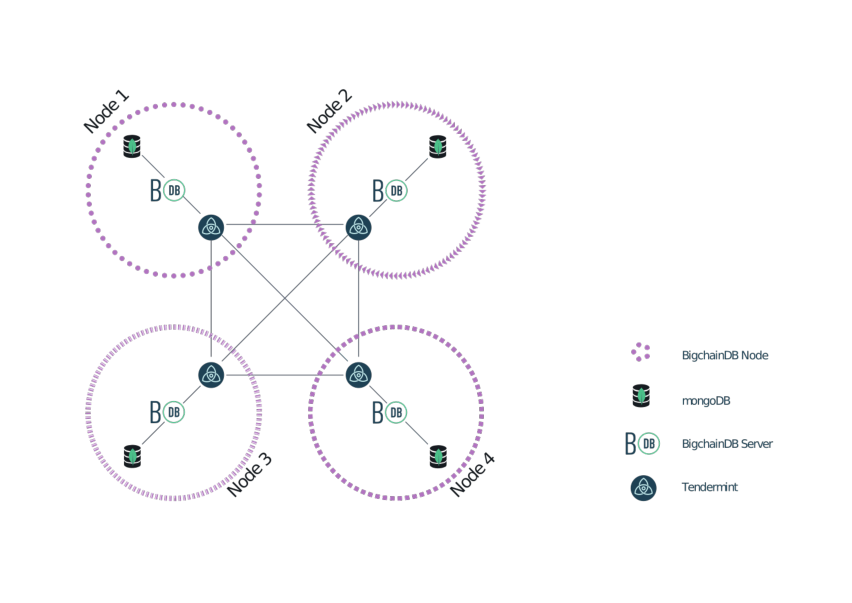
\includegraphics[width=\columnwidth]{images/bdb-arch.pdf}  
	\caption{High-Level Architecture of BigchainDB 
		2.0~\cite{bdb18d}}\label{f:bdb}
\end{figure}

\begin{figure}[!htb]
	\centering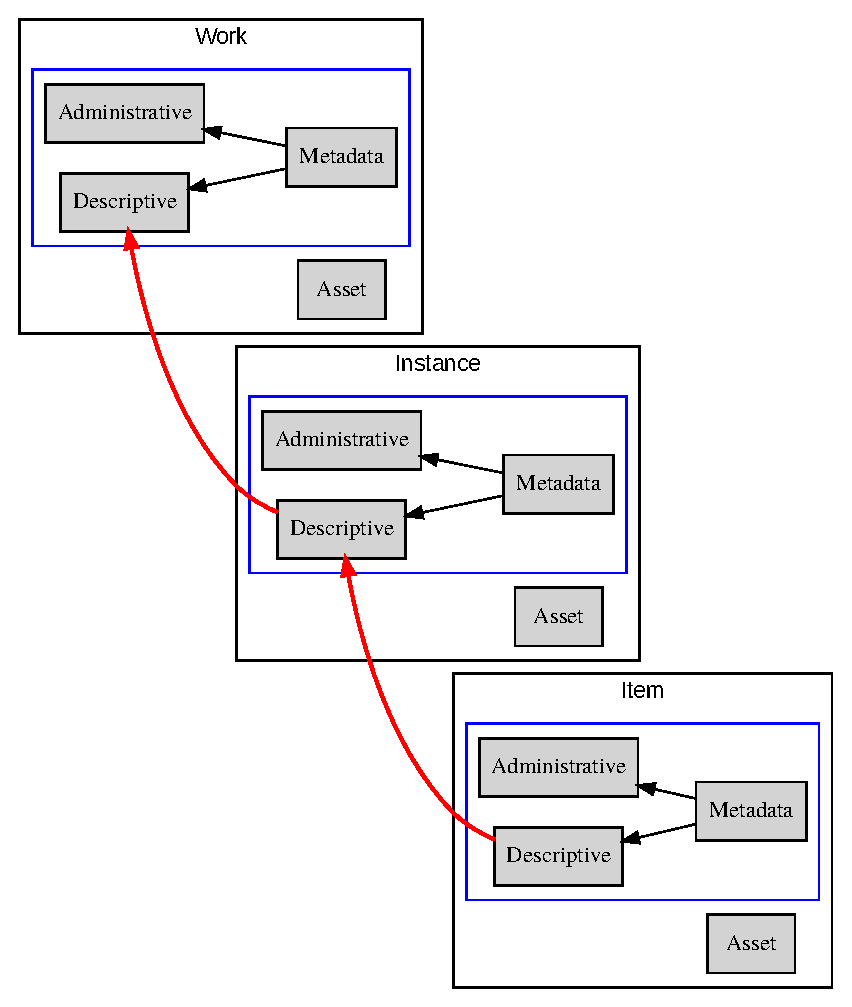
\includegraphics[width=\columnwidth]{images/assets-metadata.pdf}  
	\caption{Graph of asset and metadata objects in BigchainDB}\label{f:rbac}
\end{figure}

\begin{figure}[!htb]
	\centering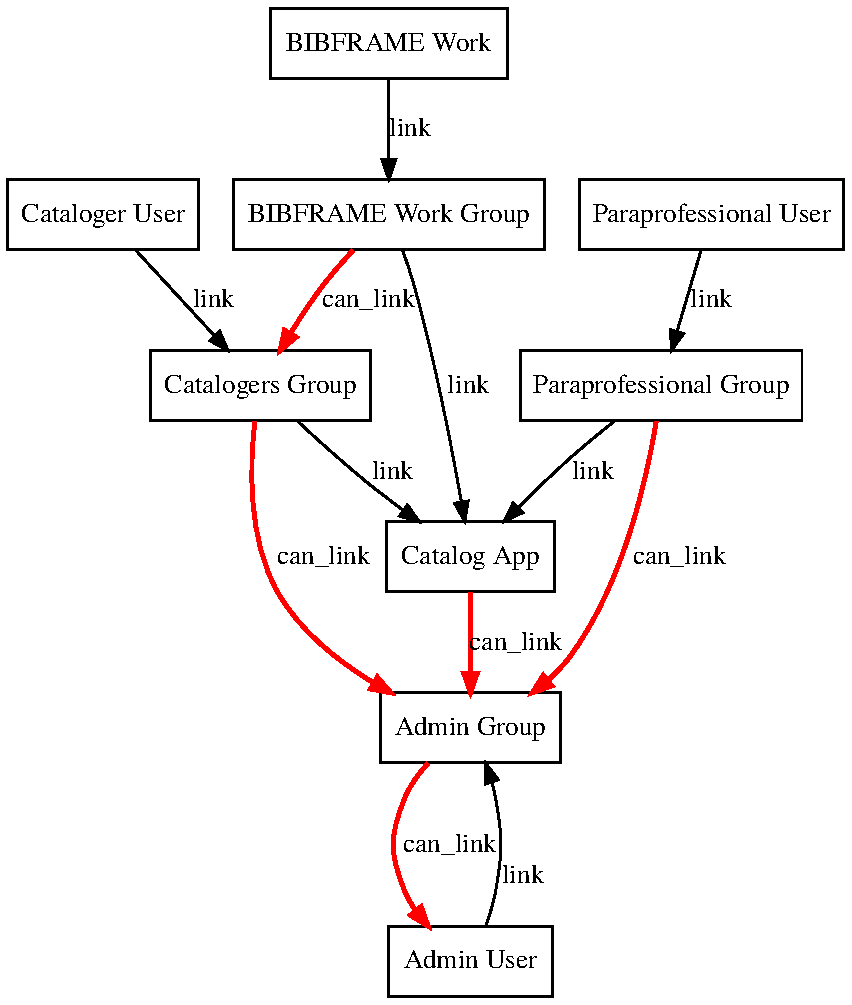
\includegraphics[width=\columnwidth]{images/rbac-graph.pdf}  
	\caption{Graph of permissions in BigchainDB using Role-Based Access 
	Control}\label{f:rbac2}
\end{figure}

\begin{figure}[!htb]
	\centering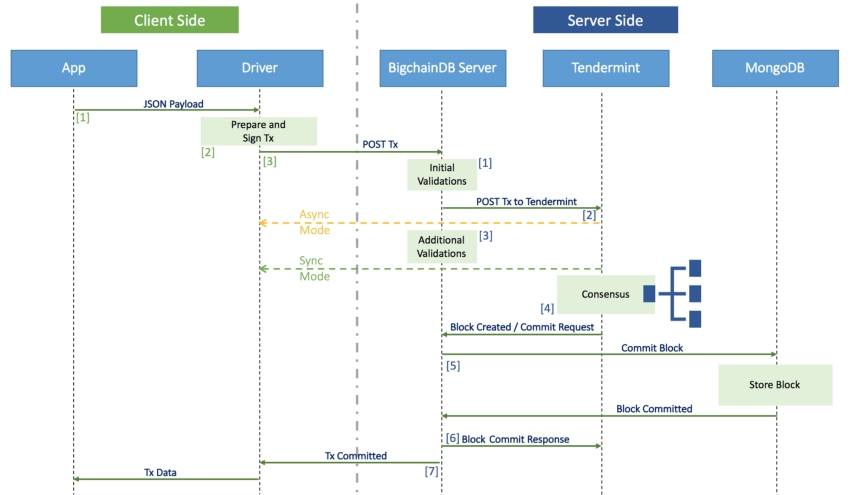
\includegraphics[width=\columnwidth]{images/bdb-seq.pdf}  
	\caption{BigchainDB Sequence Diagram~\cite{aA17}}\label{f:bdb2}
\end{figure}


\section{Conclusion}


\begin{acks}
The author would like to thank Dr.~Gregor~von~Laszewski and the i523
and i516 teaching assistants for their support and suggestions in writing
this report.
\end{acks}

\bibliographystyle{ACM-Reference-Format}
\bibliography{report} 

